\subsection{UC9 - Associazione dei predittori al flusso dati}
\begin{figure}[H]
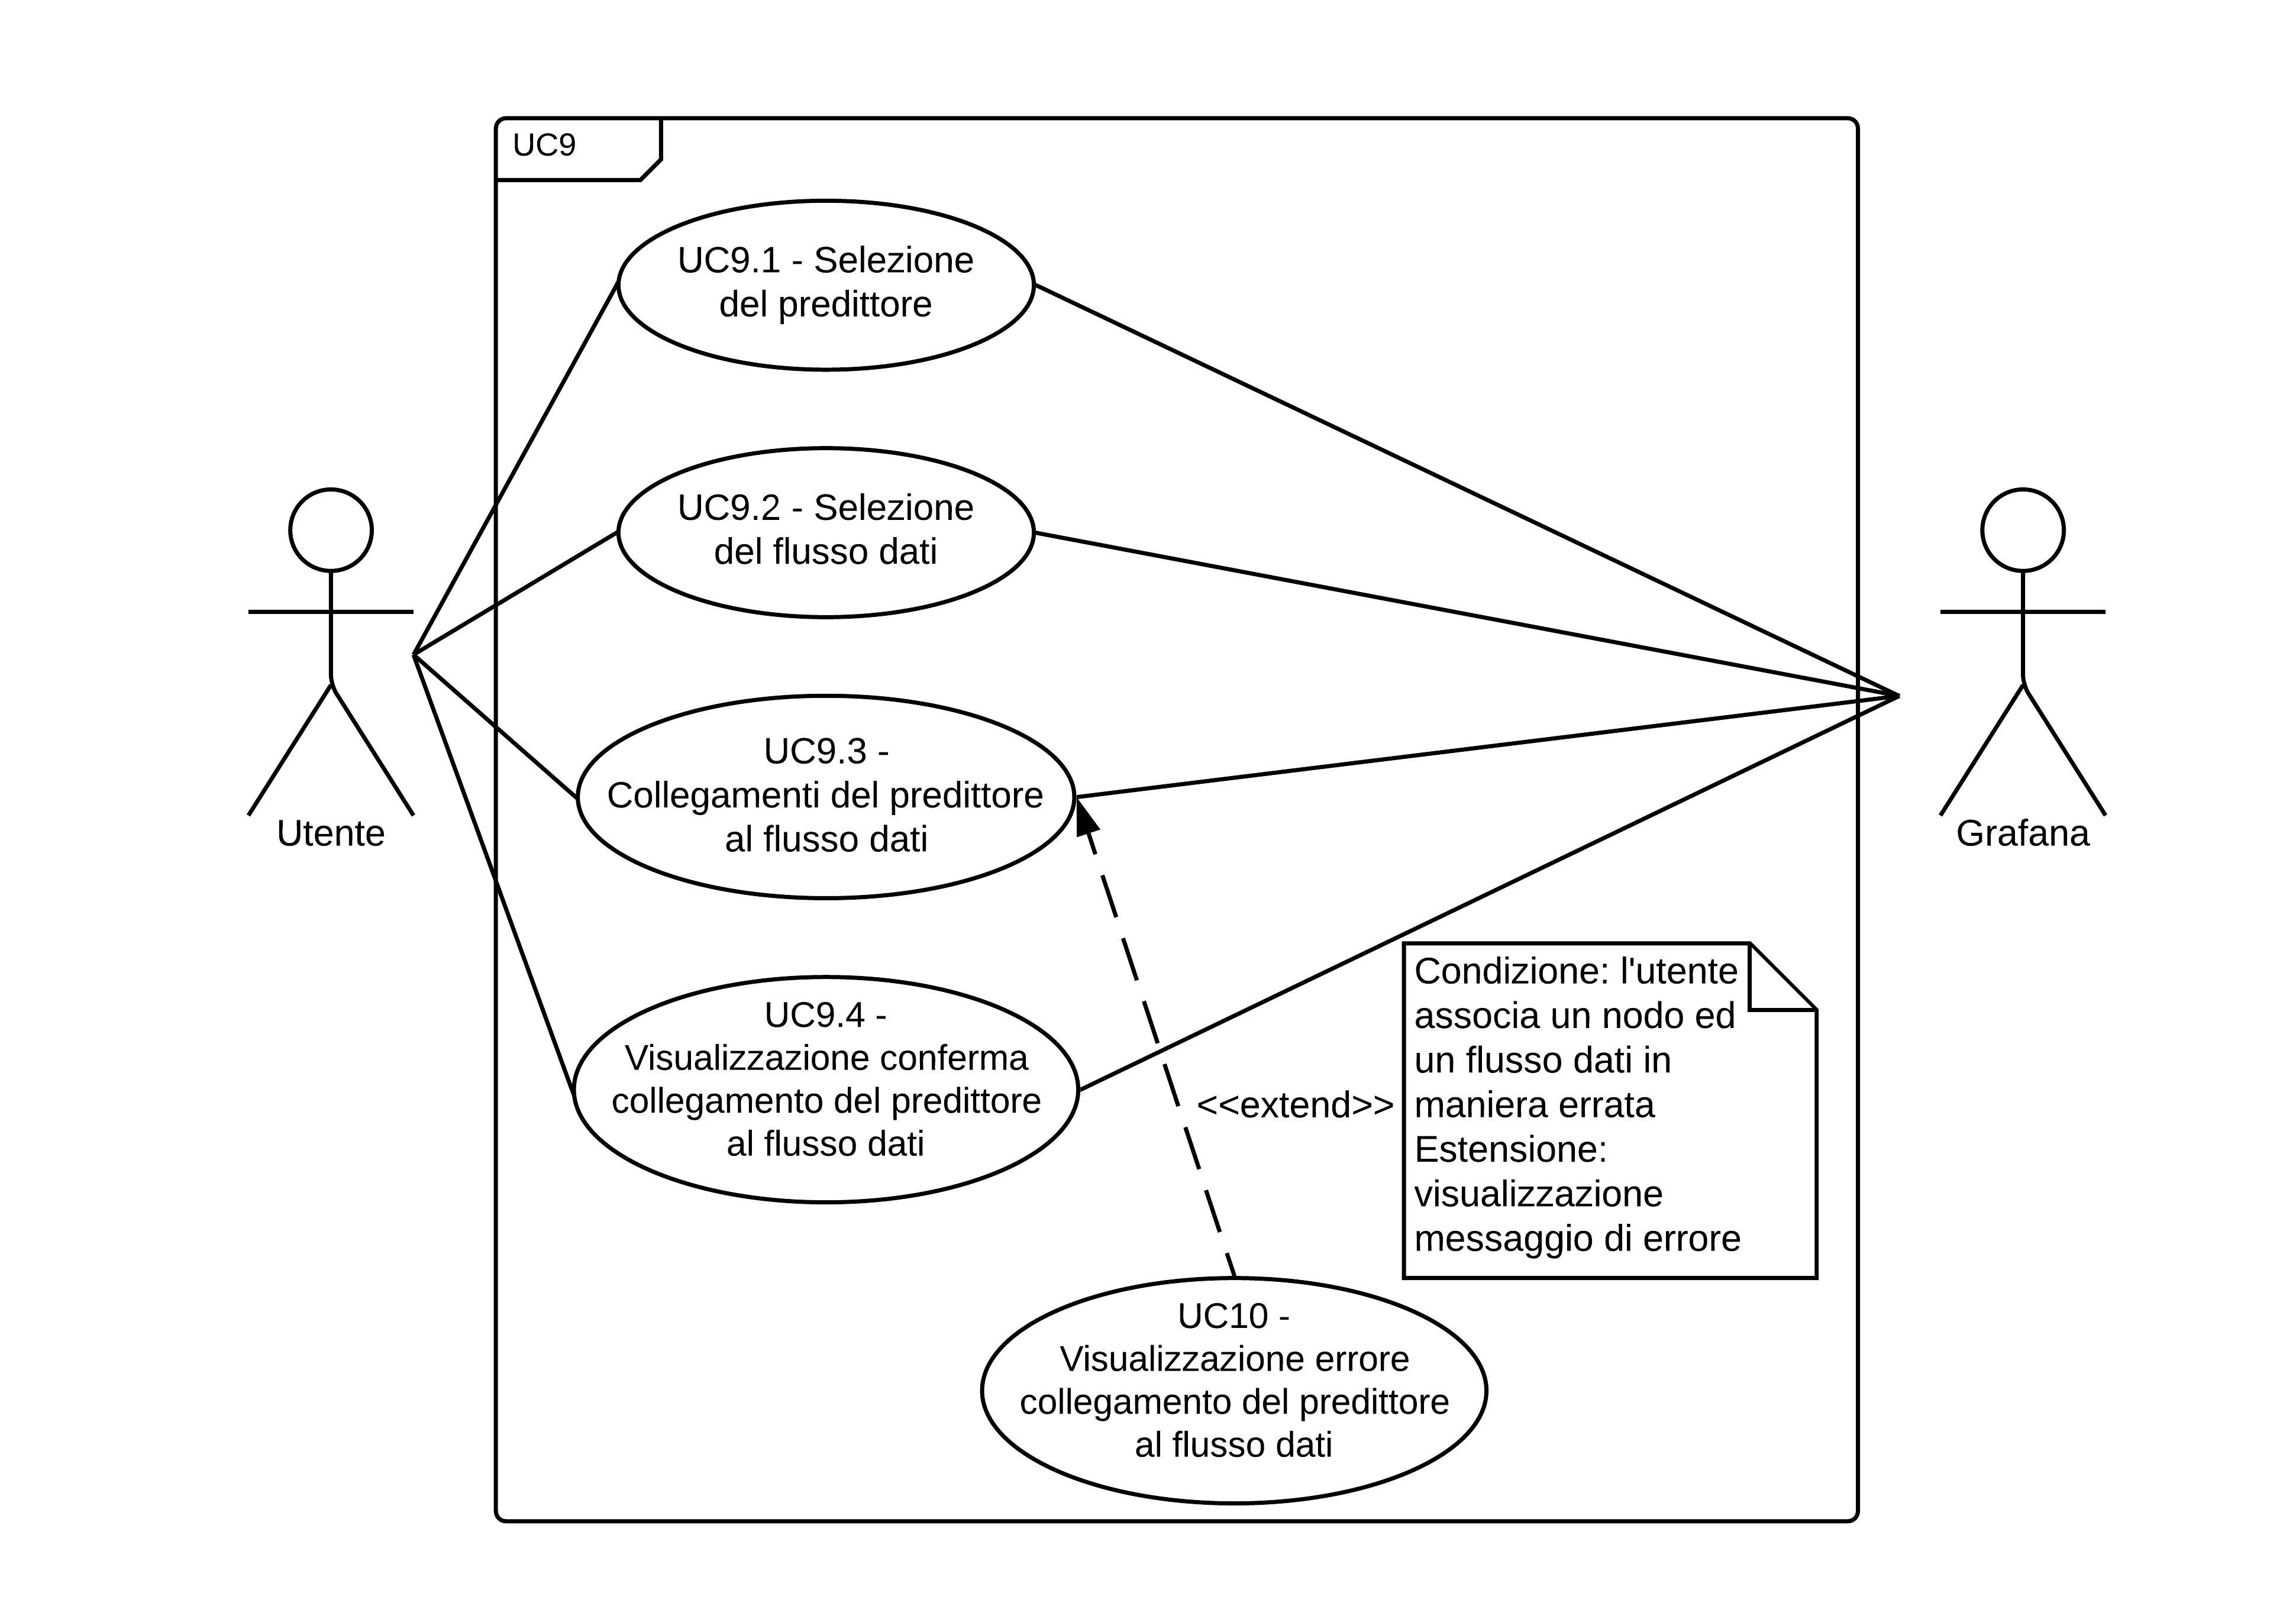
\includegraphics[width=\textwidth,height=\textheight,keepaspectratio]{img/UC9_-_Associazione_dei_predittori_al_flusso_dati.png}
\caption{Diagramma dello use case UC9}
\end{figure}
\begin{itemize}
	\item \textbf{Codice identificativo}: UC9;
	\item \textbf{Titolo}: associazione dei predittori\glosp al flusso dati;
	\item \textbf{Attori primari}: utente;
	\item \textbf{Attori secondari}: Grafana\glo;
	\item \textbf{Descrizione}: l'utente esegue l'associazione dei predittori\glosp individuati per l'attività di previsione;
	\item \textbf{Precondizioni}: l'utente è autenticato nel sistema software Grafana\glo, ha avviato il plug-in e ha caricato il file JSON con i dati di addestramento;
	\item \textbf{Postcondizioni}: i predittori\glosp sono stati associati al flusso dati con successo;
	\item \textbf{Scenario principale}: 
		\begin{enumerate}
			\item selezione del predittore\glosp (UC9.1);
			\item selezione del flusso dati (UC9.2);
			\item collegamenti del predittore\glosp al flusso dati (UC9.3);
			\item visualizzazione conferma collegamento del predittore\glosp al flusso dati (UC9.4).
		\end{enumerate}
\end{itemize}

\subsubsection{UC9.1 - Selezione del predittore}
\begin{itemize}
	\item \textbf{Codice identificativo}: UC9.1;
	\item \textbf{Titolo}: selezione del predittore\glo;
	\item \textbf{Attori primari}: utente;
	\item \textbf{Attori secondari}: Grafana\glo;
	\item \textbf{Descrizione}: l'utente seleziona il predittore\glosp tramite il plug-in;
	\item \textbf{Precondizioni}: l'utente ha avviato correttamente il plug-in;
	\item \textbf{Postcondizioni}: l'utente ha selezionato correttamente il predittore\glo;
	\item \textbf{Scenario principale}: l'utente seleziona il predittore\glosp da associare al flusso di dati.
\end{itemize}

\subsubsection{UC9.2 - Selezione del flusso dati}
\begin{itemize}
	\item \textbf{Codice identificativo}: UC9.2;
	\item \textbf{Titolo}: selezione del flusso dati;
	\item \textbf{Attori primari}: utente;
	\item \textbf{Attori secondari}: Grafana\glo;
	\item \textbf{Descrizione}: l'utente seleziona il flusso di dati tramite il plug-in;
	\item \textbf{Precondizioni}: l'utente ha avviato correttamente il plug-in;
	\item \textbf{Postcondizioni}: l'utente ha selezionato correttamente flusso dati;
	\item \textbf{Scenario principale}: l'utente seleziona il flusso dati a cui viene associato il predittore\glo.
\end{itemize}

\subsubsection{UC9.3 - Collegamenti del predittore al flusso dati}
\begin{itemize}
	\item \textbf{Codice identificativo}: UC9.3;
	\item \textbf{Titolo}: collegamenti del predittore\glosp al flusso dati;
	\item \textbf{Attori primari}: utente;
	\item \textbf{Attori secondari}: Grafana\glo;
	\item \textbf{Descrizione}: l'utente esegue il collegamento del predittore\glosp al flusso dati;
	\item \textbf{Precondizioni}: l'utente ha avviato correttamente il plug-in, ha selezionato il predittore\glosp ed il flusso dati;
	\item \textbf{Postcondizioni}: l'utente ha collegato correttamente il predittore\glosp al flusso dati;
	\item \textbf{Scenario principale}: l'utente seleziona il flusso dati a cui viene associato il predittore\glo;
	\item \textbf{Estensioni}:
	\begin{enumerate}
		\item se l'utente crea un abbinamento non valido tra un predittore\glosp ed il flusso dati viene visualizzato un messaggio di errore (UC10).
	\end{enumerate}
\end{itemize}

\subsubsection{UC9.4 - Visualizzazione conferma collegamento del predittore al flusso dati}
\begin{itemize}
	\item \textbf{Codice identificativo}: UC9.4;
	\item \textbf{Titolo}: visualizzazione conferma collegamento del predittore\glosp al flusso dati;
	\item \textbf{Attori primari}: utente;
	\item \textbf{Attori secondari}: Grafana\glo;
	\item \textbf{Descrizione}: l'utente visualizza la conferma di collegamento del predittore\glosp al flusso dati avvenuta con successo;
	\item \textbf{Precondizioni}: l'utente ha avviato il plug-in e ha eseguito il collegamento del predittore\glosp al flusso dati;
	\item \textbf{Postcondizioni}: l'utente ha visualizzato la conferma del collegamento del predittore\glosp al flusso dati;
	\item \textbf{Scenario principale}: l'utente visualizza la conferma del collegamento del predittore\glosp al flusso dati.
\end{itemize}